%!TEX root = main.tex
\section{Results}

The Dieleman model was used for both sex and speaker classification. The results are presented below.
\todo{show variance of output/compute p-values for performance difference}
\begin{table}[H]
\centering
\begin{tabular}{r|c|c}
	model & TIMIT & ELSDSR \\ \hline
	Baseline & 0.354 & 0.465 \\
	Logistic & 0.215463 & 0.020260 \\
	Dieleman & 0.102662 & 0.021708 \\
	Dieleman + Weight Decay     & 0.166033 & 0.044863 \\
	Dieleman + Scale Invariant  & 0.101394 & 0.033285 \\
	Dieleman + Offset Invariant & 0.125475 & 0.028944
\end{tabular}
\caption{misclassification rate for sex classification}
\end{table}

\begin{table}[H]
\centering
\begin{tabular}{r|c|c}
	model & TIMIT & ELSDSR \\ \hline
	Baseline & \\
	GMM on MFCC & \\
	Logistic & \\
	Dieleman & \\
	Dieleman + Weight Decay     & \\
	Dieleman + Scale Invariant  & \\
	Dieleman + Offset Invariant &
\end{tabular}
\caption{misclassification rate for speaker classification}
\end{table}

As seen the Dieleman model does not appear to be better than a simple logistic model or the GMM. Because the logistic model can be expressed as a simple neural network, we attempted to expand the logistic network with individual layers form the Dieleman network, however all configuration that uses convolutional layers performed performed similarly to the Dieleman network.

Because the Scale Invariant and Offset Invariant regularizers did not improve the results on sex or speaker classification, the regularizers under optimal conditions. These conditions are synthetically constructed 2 dimensional datasets. \todo{elaborate}

\begin{figure*}[h]
	\centering
	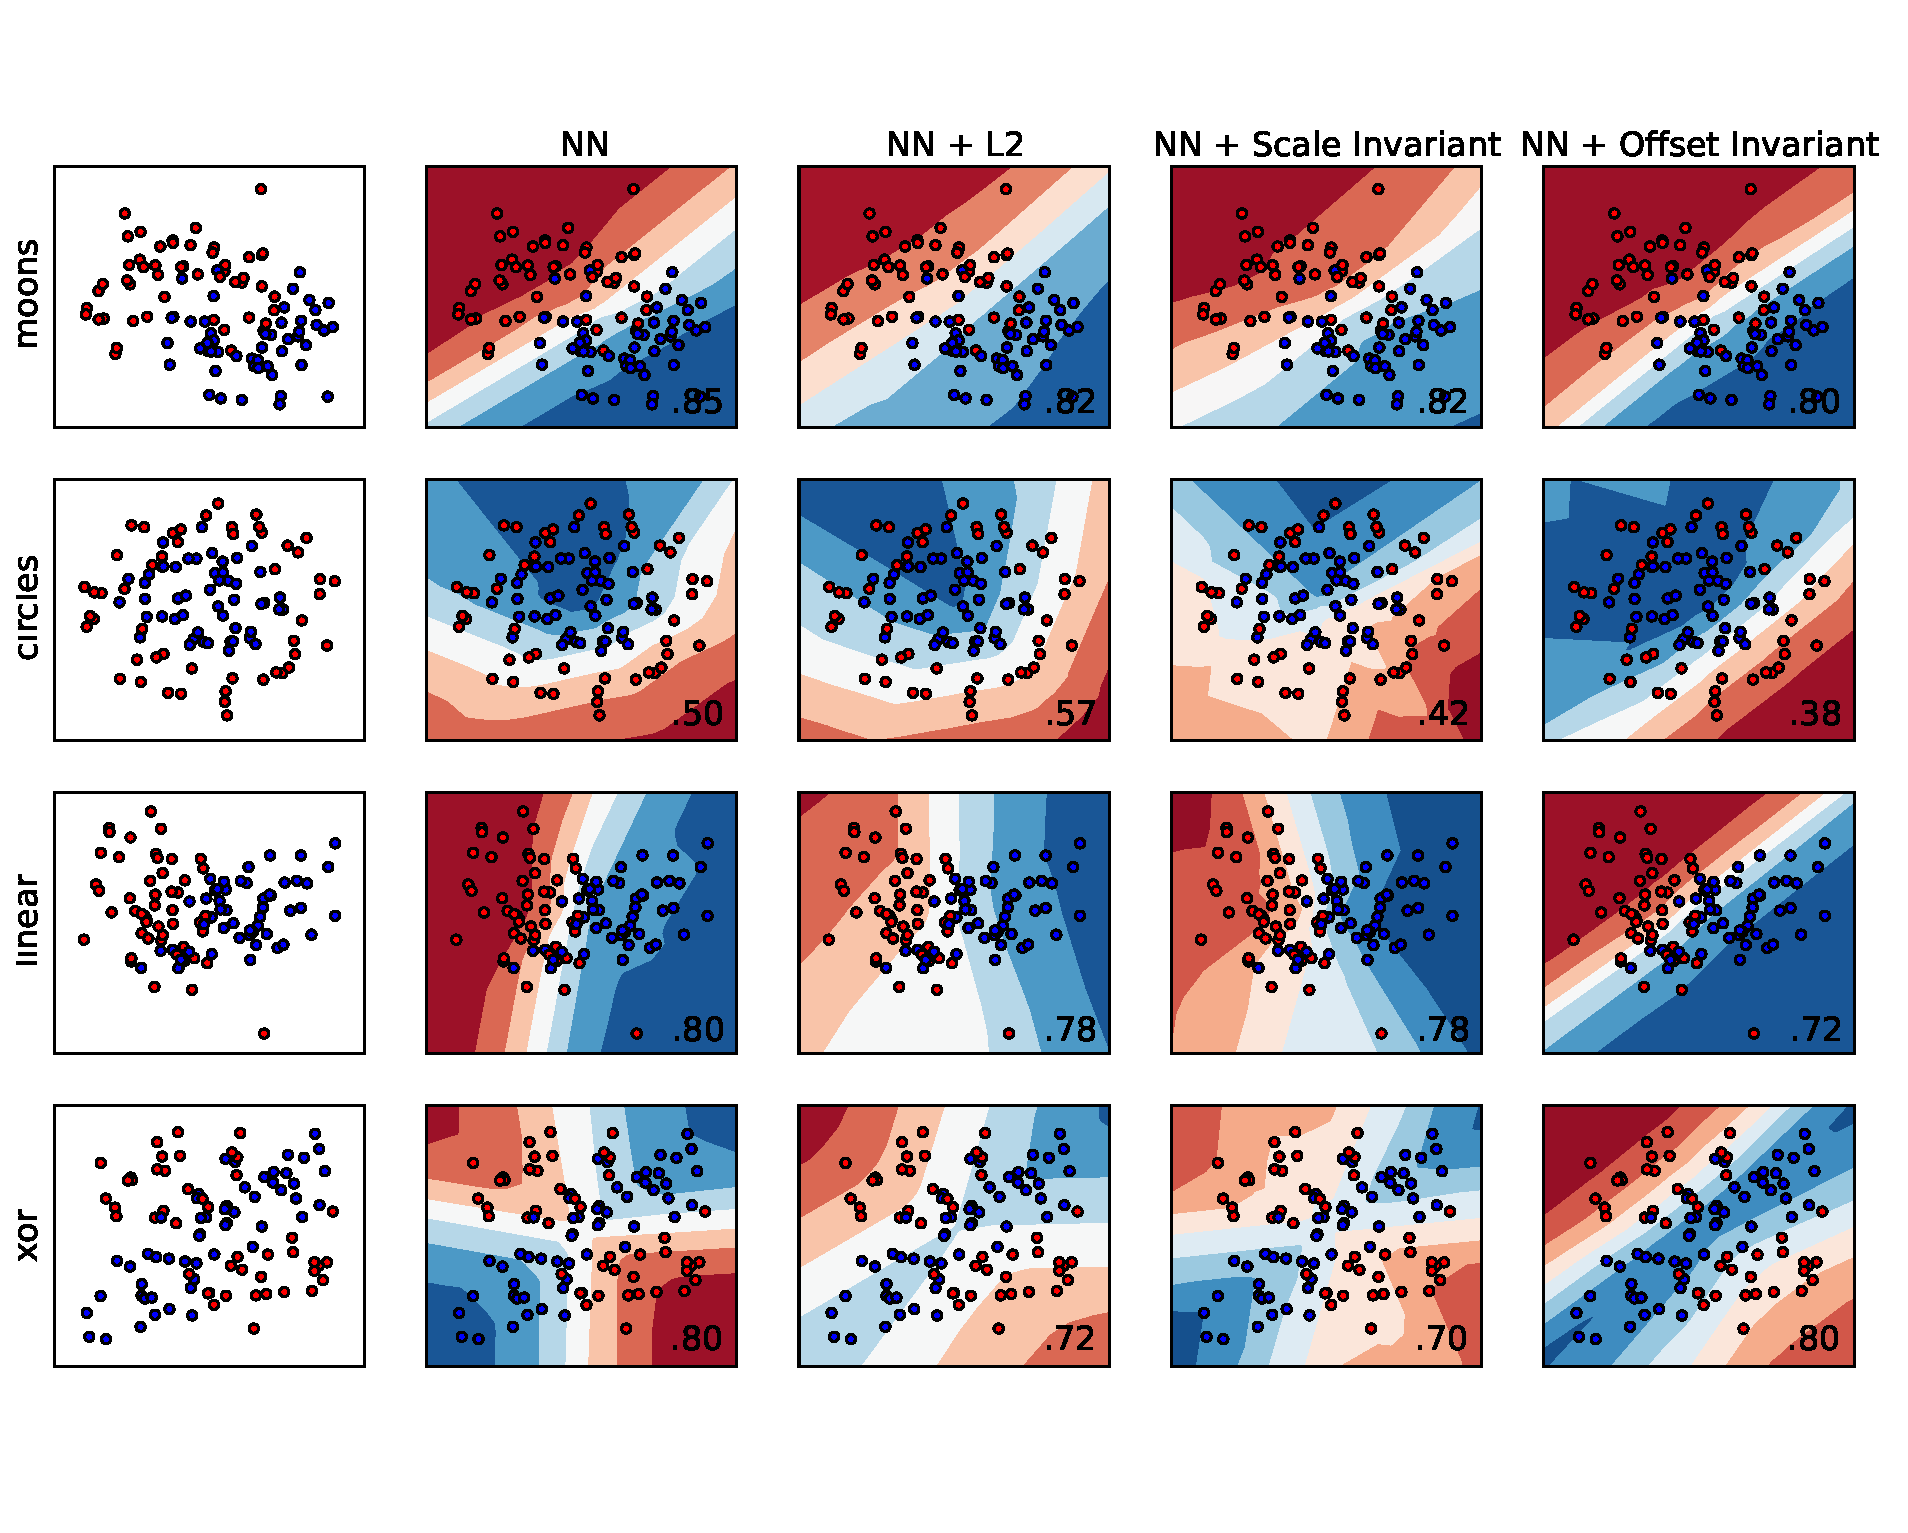
\includegraphics[width=0.7\textwidth, trim = 0 2.2cm 0 2cm, clip]{plots/2d_classifier}
	\caption{Observations and contour plot of the class probability function for each classifier and dataset.}
\end{figure*}

100 datasets for each data generator was then created to determine if are any statistical difference in the performance.

\begin{figure}[H]
	\centering
	\includegraphics[width=0.5\textwidth]{plots/2d_significant}
	\caption{Boxplot of performance on the 100 datasets for each data generator and classification model.}
\end{figure}


•Objective presentation of key results, without interpretation (text and tables
and figures)
•Important negative results should also be reported
